\documentclass[titlepage]{ltjsarticle}
% ページスタイル
\pagestyle{headings}
% 数式
\usepackage{amsmath,amsfonts}
\usepackage{bm}
% 数式
\usepackage{amsthm}
\usepackage{amssymb}
\usepackage{amsfonts}
\usepackage{bm}
\usepackage{derivative}
% 式番号を途中でふらない(参照するものだけ参照する)
\usepackage{mathtools}
\mathtoolsset{showonlyrefs=true}


% 数式をすべてdisplaystyleにする。
\everymath{\displaystyle}
\usepackage{bookmark}
\hypersetup{unicode,bookmarksnumbered=true,hidelinks,final}
% mysimpleboxの設定
\usepackage{tcolorbox}
\tcbuselibrary{skins}
\newtcolorbox{mysimplebox}[1]{%
colframe=black,colback=white,
coltitle=black,colbacktitle=white,
boxrule=0.8pt,arc=0mm,
fonttitle=\sffamily\bfseries,
enhanced,
attach boxed title to top left={xshift=10mm ,yshift=-3mm},
boxed title style={frame hidden},
title=#1}
% Pythonでのグラフ描画をインポートするために必要なパッケージ
\usepackage{graphicx}
\usepackage[utf8]{inputenc}
\usepackage{pgfplots}
\pgfplotsset{compat=1.18}
% braket 記法を用いる。
\usepackage{physics2}
\usephysicsmodule{braket}
\newcommand{\mel}[3]{\braket[3]{#1}{#2}{#3}}
\newcommand{\ev}[1]{\braket[1]{#1}}
\begin{document}
\title{物性物理学}
\author{寺崎一郎}
\date{\today}
\maketitle  

\section{第3回}
前回の復習から、考える。
\begin{enumerate}
  \item 自由電子は\(e^{ikx}\)でエネルギーは、\(\frac{\hbar^2k^2}{2m}\)運動量は\(\hbar k\)となる。
  \item PBCCでは\(L=Na\)となり、
  \begin{equation}
    \varphi(x) = \varphi(x+L) = \varphi(x+Na)
  \end{equation}
  となり、\(k=\frac{2 \pi}{Na}\)の整数\(\frac{1}{\sqrt{L}}e^{ikx}\)となる、
  \item 第一BZについては、
  \begin{equation}
    -\frac{\tau}{a} \le k \le \frac{\pi}{a}
  \end{equation}
  となる。独立な\(k\)のセットである。
  \item \(a\)の並進対称性としては、
  \begin{align}
    \hat{T} \varphi(x) &= \varphi(x+a) = \varphi(x) \\
    \hat{T} \varphi(k) &= e^{ika} \varphi(k)
  \end{align}
  となる。同じ固有値\(e^{ika}\)をもつ\(k\)の組
  \begin{equation}
    -\frac{\pi}{a} \le k \le \frac{\pi}{a}
  \end{equation}
  ととると、
  \begin{align}
    k = k_0 + k_m \\
    k_m = \frac{2 \pi}{a}m
  \end{align}
  となる。
\end{enumerate}
\subsubsection{二次元の自由電子}
二次元の自由電子では、
\begin{equation}
  -\frac{\hbar^2}{2m} \left( \pdv[order=2]{}{x} + \pdv[order=2]{}{y} \right)\varphi(x.y) = \varepsilon \varphi(x,y)
\end{equation}
となり、\(\varphi(x,y) = X(x)Y(y)\)と仮定する。
すると、
\begin{equation}
  - \frac{\hbar^2}{2m} \pdv[order=2]{X}{x}Y(y) - \frac{\hbar^2}{2m} X(x) \pdv[order=2]{Y}{y} = \varepsilon X(x)Y(y)
\end{equation}
となることから、辺々を\(XY\)で割ると、
\begin{equation}
  X \propto e^{ik_x x}, Y \propto e^{ik_y y}
\end{equation}
となることから、\(\varepsilon_x = \frac{\hbar^2 k^2}{2m},\varepsilon_y = \frac{\hbar^2 k^2}{2m},\varepsilon_y\)となる。

ここから、
\begin{equation}
  \exp \left( \bm{k}\cdot \bm{\Gamma} \right) = \exp\left( k_x x + k_y y \right)
\end{equation}
となる。
エネルギーとしては、
\begin{equation}
  \varepsilon = \frac{\hbar^2}{2m}(k_x^2 + k_y^2)
\end{equation}
となる。
さらに、運動量は、
\begin{equation}
  \bm{p} = \hbar \bm{k} = (\hbar k_x, \hbar k_y)
\end{equation}
となる。
さらに、PBCは、
\begin{equation}
  \varphi(x,y) = \varphi(x+L,y) = \varphi(x,y+L)
\end{equation}
となることがわかる。\(e^{ik_xL}=e^{ik_yL}=1\)となる。ことから、規格化されて、
\begin{equation}
  k_x = \frac{2 \pi}{L}n_x, k_y = \frac{2 \pi}{L}n_y
\end{equation}
となり、規格化して、\(\int_{0}^{L}\int_{0}^{L}\odif{x,y}|\varphi|^2 =1\)となることから、
\(A=\frac{1}{L}\)をとり、
\begin{equation}
  \varphi(x,y) = \frac{1}{\sqrt{L^2}}e^{i\bm{k}\cdot \bm{r}}
\end{equation}
となるために、第一BZは、\(-\frac{\pi}{a}\le k_x \le \frac{\pi}{a},-\frac{\pi}{a}\le k_y \le \frac{\pi}{a}\)となる。

\subsubsection{\(a\)の並進対称性}

\(a\)の並進対称性は、
\begin{align}
  \hat{T}_x \varphi(x,y) &= \varphi(x+a,y) = \varphi(x,y) \\
  \varphi(x,y) & = \frac{1}{L}e^{i \bm{k}\cdot \bm{r}}\\
  \hat{T}_x \varphi(x,y) & = e^{ik_x a} \varphi(x,y)\\
  \varphi(x+a,y) & = \frac{1}{L} e^{i \bm{k}\cdot \bm{r}} \\
  & = e^{ik_x a} \varphi(x,y)
\end{align}
となることから、
第一BZ内の\(k_x\)に対して、
\begin{equation}
  k_x + k_{m_x}
\end{equation}
は、\(\hat{T}_x\)に対して、同じ固有値\(e^{ik_x a}\)を与える。
\begin{equation}
  K_{m_x} = \frac{2 \pi}{a}m_x
\end{equation}
ただし、\(m_x\)は整数である。どうように\(k_{m_y}=\frac{2\pi}{a}m_y\)が定義できる。

\subsubsection{逆格子}
実格子は\(a\)ずつの点であるが、逆格子は\(\frac{2\pi}{a}\)ずつの点のことである。

二次元の場合には、逆格子は\(-\frac{\pi}{a}\le k_x \le \frac{\pi}{a},-\frac{\pi}{a}\le k_y \le \frac{\pi}{a}\)が第一BZになり、次は、\(k_x = \pm \frac{2\pi}{a},k_y = \pm \frac{2 \pi}{a}\)wそれぞれ結んだひし形から第一BZを引いた値である。

さてもう少し抽象的なことをいおう。
まずは実格子に必要なベクトルのことを
\begin{equation}
  \begin{cases}
    \bm{a}_1 = a \bm{e}_x \\
    \bm{a}_2 = a \bm{e}_y
  \end{cases}
\end{equation}
となる。そして、逆格子は
\begin{equation}
  \begin{cases}
    \bm{b}_1 = \frac{2\pi}{a}\bm{e}_x = \frac{2\pi}{a} \bm{e}_{k_x} \\
    \bm{b}_2 = \frac{2\pi}{a}\bm{e}_y= \frac{2\pi}{a} \bm{e}_{k_y}
  \end{cases}
\end{equation}
となる。

\subsubsection{一般の二次元格子と逆格子}
一般の二次格子を拡張しておく。
\begin{equation}
  |\bm{a}_1 | = | \bm{a}_2 | 
\end{equation}
となり、\( \bm{a}_1\)と\(\bm{a}_2\)は直交しない。
対応する\(\bm{b}_1,\bm{b}_2\)はどう取ったらいいか?
一次元の場合には、
\begin{equation}
  \exp\left( ika \right) = \exp\left( i \left( k + k_m \right)a \right)
\end{equation}
となり、\(k_m = \frac{2\pi}{a}m\)となる、
二次元正方格子の場合には、
\begin{equation}
  \exp \left( i \bm{k} \cdot \bm{r} \right) \to \exp\left( \bm{k}\left( \bm{r} + \bm{a} \right) \right)  
\end{equation}
となる。ここから、\(\bm{K}\cdot \bm{a}\)が\(2 \pi\)の整数倍になるようにする。
ここで、\(\bm{a}_1\cdot \bm{b}_1 = 2\pi,\bm{a}_1 \cdot \bm{b}_2= \bm{a}_2 \cdot \bm{b}_1 = 0, \bm{a}_2 \cdot \bm{b}_2 = 2\pi\)となることを用いて、
\begin{align}
  \bm{k} & = n_1 \bm{b}_1 + n_2 \bm{b}_2 \\
  \bm{k}\cdot \bm{a} & = (m_1 \bm{b}_1 + m_2 \bm{b}_2) \cdot (n_1 \bm{a}_1 + n_2 \bm{a}_2) \\
   & = m_1 n_1 \bm{a}_1 \bm{b}_1 + m_2 n_2 \bm{a}_2 \bm{b}_2 + m_1 n_2 \bm{a}_1 \bm{b}_2 + m_2 n_1 \bm{a}_2 \bm{b}_1\\
   & = 2 \pi (m_1 n_1 + m_2 n_2)
\end{align}

これから、これを拡張すると、一般の\(\bm{a}_1,\bm{a}_2\)に対して、
\begin{equation}
  \begin{cases}
    \bm{a}_1 \cdot \bm{b}_1 = 2 \pi \\
    \bm{a}_1 \cdot \bm{b}_2 =\bm{a}_2 \cdot \bm{b}_1 =0 \\
    \bm{a}_2 \cdot \bm{b}_2 = 2 \pi
  \end{cases}
\end{equation}
となるように\(\bm{b}_1,\bm{b}_2\)となるように決める。

第三回の画像を見ながら
逆格子の世界には色がない。違う原子があったから撮って色が違うわけではない。色が互い違いにちがうときに、同じところに戻って来るのは\(2a\)である。

逆格子の世界に種類はないので、最小になるように選ぶ。

\(\bm{a}_i\)を基本並進ベクトルであり\(\bm{b}_j\)は基本逆格子ベクトルであり、\(\bm{a}_i \bm{b}_j=2\pi \delta_{ij}\)となる。

\section{四回目}

\subsubsection{ブラケット記法}
\(\ket{n}\)状態の\(n\)に対するケットベクトルは縦ベクトルであり、\(\bra{m}\)は、
\begin{equation}
  \braket{m}{n} = \int \odif[order=3]{r} \varphi_m^*(\bm{r})\varphi_n(\bm{r})
\end{equation}
となり、
\begin{equation}
  \mel{m}{\hat{A}}{n} = \int \odif[order=3]{r} \varphi_m^*(\bm{r})\hat{A}\varphi_n(\bm{r}) = A_{mn}
\end{equation}
となり、行列要素となる。
正規直交基底としては、
\begin{equation}
  \braket{m}{n} = \delta_{mn}
\end{equation}
となり、完全系条件は、
\begin{equation}
  \sum_{n} \ket{n}\bra{n} = 1
\end{equation}
となる。

\subsubsection{変分法}
変分法とは、
\begin{equation}
  \hat{H} \ket{n} = \varepsilon_n \ket{n}
\end{equation}
としてあげると、\(\braket{m}{n} = \delta_{mn}\)となる。

個々かから任意の状態\(\ket{\varphi} = \sum_n c_n \ket{n}\)
とすると、
\begin{align}
  \mel{\varphi}{\hat{H}}{\varphi}  & = \sum_{m,n} c_m^* c_n \mel{m}{\hat{H}}{n} = \sum_{m,n} c_m^* c_n \varepsilon_n \\
  & = \sum_{n} |c_n|^2 \varepsilon_n \\
  & = \sum_n \varepsilon_n |c_n|^2
\end{align}
となる。\(\varepsilon_n\)を\(\varepsilon_0\)に置き換えることである。
すると、
\begin{equation}
  \mel{\varphi}{\hat{H}}{\varphi}  = \sum_n \varepsilon_n |c_n|^2 \ge \varepsilon_0 \sum_n |c_n|^2 = \varepsilon_0
\end{equation}
となるので、近似の波動関数は基底状態よりも大きなエネルギー状態を持つということである。


\(\ket{\varphi}\)を見つけて。低い値が見つかればそれは基底状態であることがわかる。



\tikzset{every picture/.style={line width=0.75pt}} %set default line width to 0.75pt        

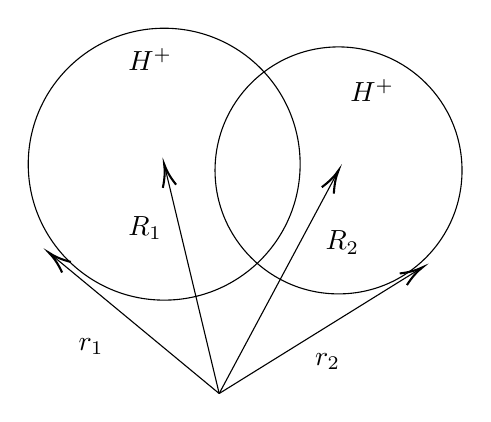
\begin{tikzpicture}[x=0.75pt,y=0.75pt,yscale=-1,xscale=1]
%uncomment if require: \path (0,235); %set diagram left start at 0, and has height of 235

%Shape: Circle [id:dp19702952708400878] 
\draw   (188,89.5) .. controls (188,53.33) and (217.33,24) .. (253.5,24) .. controls (289.67,24) and (319,53.33) .. (319,89.5) .. controls (319,125.67) and (289.67,155) .. (253.5,155) .. controls (217.33,155) and (188,125.67) .. (188,89.5) -- cycle ;
%Shape: Circle [id:dp25568216024195967] 
\draw   (278,92.5) .. controls (278,59.64) and (304.64,33) .. (337.5,33) .. controls (370.36,33) and (397,59.64) .. (397,92.5) .. controls (397,125.36) and (370.36,152) .. (337.5,152) .. controls (304.64,152) and (278,125.36) .. (278,92.5) -- cycle ;
%Straight Lines [id:da15186294309395065] 
\draw    (280,200) -- (376.3,140.22) ;
\draw [shift={(378,139.17)}, rotate = 148.17] [color={rgb, 255:red, 0; green, 0; blue, 0 }  ][line width=0.75]    (10.93,-3.29) .. controls (6.95,-1.4) and (3.31,-0.3) .. (0,0) .. controls (3.31,0.3) and (6.95,1.4) .. (10.93,3.29)   ;
%Straight Lines [id:da17817439842273108] 
\draw    (280,200) -- (199.54,133.44) ;
\draw [shift={(198,132.17)}, rotate = 39.6] [color={rgb, 255:red, 0; green, 0; blue, 0 }  ][line width=0.75]    (10.93,-3.29) .. controls (6.95,-1.4) and (3.31,-0.3) .. (0,0) .. controls (3.31,0.3) and (6.95,1.4) .. (10.93,3.29)   ;
%Straight Lines [id:da24566407788550237] 
\draw    (280,200) -- (336.56,94.26) ;
\draw [shift={(337.5,92.5)}, rotate = 118.14] [color={rgb, 255:red, 0; green, 0; blue, 0 }  ][line width=0.75]    (10.93,-3.29) .. controls (6.95,-1.4) and (3.31,-0.3) .. (0,0) .. controls (3.31,0.3) and (6.95,1.4) .. (10.93,3.29)   ;
%Straight Lines [id:da8593339210624895] 
\draw    (280,200) -- (253.97,91.44) ;
\draw [shift={(253.5,89.5)}, rotate = 76.51] [color={rgb, 255:red, 0; green, 0; blue, 0 }  ][line width=0.75]    (10.93,-3.29) .. controls (6.95,-1.4) and (3.31,-0.3) .. (0,0) .. controls (3.31,0.3) and (6.95,1.4) .. (10.93,3.29)   ;

% Text Node
\draw (211,172.4) node [anchor=north west][inner sep=0.75pt]    {$r_{1}$};
% Text Node
\draw (325,179.4) node [anchor=north west][inner sep=0.75pt]    {$r_{2}$};
% Text Node
\draw (235,113.4) node [anchor=north west][inner sep=0.75pt]    {$R_{1}$};
% Text Node
\draw (330,120.4) node [anchor=north west][inner sep=0.75pt]    {$R_{2}$};
% Text Node
\draw (235,32.4) node [anchor=north west][inner sep=0.75pt]    {$H^{+}$};
% Text Node
\draw (342,47.4) node [anchor=north west][inner sep=0.75pt]    {$H^{+}$};


\end{tikzpicture}

となり、画像の中の文字はすべてベクトルとして考える。
ここで、水素原子のハミルトニアンを考えると、
\begin{equation}
  \hat{H} = -\frac{\hbar^2}{2m} (\nabla_1^2 + \nabla_2^2) - \frac{e^2}{4\pi \varepsilon_0 } \sum^2_{i=1} \sum^2_{j=1} \frac{1}{|\bm{r}_i-\bm{R}_j|} +  \frac{e^2}{4\pi \varepsilon_0 |\bm{r}_i-\bm{r}_j|}
\end{equation}
となり、\(H^+\)からの引力と電子同士の斥力の輪でわかる。
\(\bm{r}_1\)に注目し、\(\bm{r}_2\)は平均値\(\ev{\bm{r}_2}\)でおきかえる。

すると、
\begin{equation}
  \hat{H}_2 = -\frac{\hbar^2}{2m} \nabla_1^2 -\frac{e^2}{4\pi \varepsilon_0} \left( 
    \frac{1}{|\bm{r}_1-\bm{R}_1|} + \frac{1}{|\bm{r}_1-\bm{R}_2|} 
   \right) 
   + \frac{e^2}{4\pi \varepsilon_0} \frac{1}{|\bm{r}_1-\ev{\bm{r}_2}|}
\end{equation}
となる。

試行関数を使ってみる。
\begin{equation}
  \ket{\varphi} = c_1 \ket{1} + c_2 \ket{2}
\end{equation}
となる。ここで、\(\ket{c_1}\)は原子1の1s軌道であり、\(\ket{c_2}\)は原子2の1s軌道である。
水素分子の変分法としては、電子1は原子1の1s軌道であるか?原子2の1s軌道のどりかということである。


変分法の肝はtrial functionとして、求まったもので基底状態のエネルギーを求めることである。

この時、\(\ket{1}\)を\(\ket{\varphi}\)にかける
\begin{align}
  \mel{1}{\hat{H}_2}{\varphi}  & = \mel{1}{\hat{H}_2}{1}c_1 + \mel{1}{\hat{H}_2}{2}c_2\\
  & = \varepsilon c_1 + s\varepsilon c_2
\end{align}
となるはずである。ここで、。\(\mel{1}{\hat{H}}{2}=t\)である。


この時に、
\begin{align}
  \mel{\varphi}{\hat{H}_2}{\varphi} & = \int \odif[order=3]{r} \phi^\ast \left( -\frac{\hbar^2}{2m}\nabla^2_1 + \frac{e^2}{4\pi \varepsilon}\frac{1}{|\bm{r}_1-\bm{R_1}|} \right) \varphi + 
  \int \odif[order=3]{r} \phi^\ast \left( \frac{-e^2}{4\pi \varepsilon}\frac{1}{|\bm{r}_1-\bm{R_2}|}+ \frac{e^2}{4\pi \varepsilon}\frac{1}{|\bm{r}_1-\ev{\bm{r_2}}|} \right) \varphi \\
  & \simeq  \int \odif[order=3]{r} \phi^\ast \left( -\frac{\hbar^2}{2m}\nabla^2_1 + \frac{e^2}{4\pi \varepsilon}\frac{1}{|\bm{r}_1-\bm{R_1}|} \right) \varphi + 0
\end{align}

電子の位置に対して対称なハミルトニアンであるために、電子1が原子1にいてさらに電子2モ電子2にいるような確率はほとんど0としてよい。すると、\(\ev{\bm{r}_2} \simeq \bm{R}_2\)であるから、第二項は0としてもよい。そして第一項は\(\varepsilon_{1s}\)と同じ。
ここから、まったく同様に\(\ket{2}\)を使うと、

\begin{equation}
  \begin{cases}
    c_1 \varepsilon_{1s} + c_2 t = c_1 \varepsilon  + c_2 \varepsilon s\\
    c_1 t + c_2 \varepsilon_{1s} = c_1 \varepsilon s + c_2 \varepsilon
  \end{cases}
\end{equation}
この解の非自明なものを考えると、
\begin{equation}
  \varepsilon = \frac{\varepsilon_{1s}\pm t}{1\pm s}
\end{equation}
となる。
\(t= \mel{1}{\hat{H}_2}{2}\)1s軌道の場合ならマイナスである。

重なった時の波動関数の+とマイナスについて考える。
簡単のために、\(s=0\)とすると。\(\varepsilon_{12}+t\)に対して、\(c_1=c_2=\frac{1}{\sqrt{2}}\)であり\(\varepsilon_{12}-t\)に対して\(c_1=-c_2 = \frac{1}{\sqrt{2}}\)となることがw耀。
第一励起状態は、\(\varepsilon_{12}+t\)となり、
\begin{align}
  \begin{cases}
    \varepsilon_{12} + t & \frac{1}{\sqrt{2}}\left( \ket{1} + \ket{2} \right) \text{結合軌道}\\
    \varepsilon_{12} - t & \frac{1}{\sqrt{2}}\left( \ket{1} - \ket{2} \right) \text{反結合軌道}
  \end{cases}
\end{align}

\subsubsection{水素の一次元結合}
格子間隔は\(a\)としよう。
\begin{equation}
  \hat{H}_N = - \frac{\hbar^2}{2m} \nabla_1^2 - \frac{e^2}{4\pi \varepsilon_0} \frac{1}{|\bm{r}_1- n\bm{a}|} + \frac{e^2}{4\pi \varepsilon_0} \sum^N_{n=1} \frac{1}{|\bm{r}_1-\ev{\bm{r}_2}|}
\end{equation}
となる。
\begin{equation}
  \hat{H}\ket{\varphi} = \varepsilon \ket{\varphi}
\end{equation}
となり、\(\ket{\varphi} = \sum_{n=1}^{N}c_n \ket{n}\)となり、
左から\(\bra{m}\)を書けると、前回とまったく同じ議論をすれば、
\begin{align}
  \mel{n}{\hat{H}_N}{n} = \varepsilon_{1s} \\
  \braket{m}{n} = 1 \\
  \mel{m}{\hat{H}_N}{n} = t (m=n \pm 1) \\
  \braket{m}{n} = s (m = n \pm 1) \\
  \mel{m}{\hat{H}_N}{n} = \mel{m}{\varepsilon}{\varphi}
\end{align}
となる。
ここから、
\begin{equation}
  \sum_{n=1}^{N}c_n \mel{m}{\hat{H}}{n} = \varepsilon \sum_{n=1}^{N}c_n \braket{m}{n}
\end{equation}
となることから
\begin{equation}
  t c_{m-1} + \varepsilon_{1s} c_m + t c_{m+1}  = \varepsilon c_m + \varepsilon s c_{m-1} + \varepsilon s c_{m+1}
\end{equation}
となり、連戦振動の回と波動の解を持つ。
ここで数理物理学で考えたことを考えると、
\begin{equation}
  c_m = e^{ikam}
\end{equation}
を代入してあげると、
\begin{equation}
  t e^{-ika} + \varepsilon_{1s} + t e^{ika} = \varepsilon + \varepsilon s e^{-ika} + \varepsilon s e^{ika}
\end{equation}
からエネルギーを求めることは簡単で、実数部分をとってあげると
\begin{equation}
  \varepsilon = \frac{\varepsilon_{12}+2t \cos (ka)}{1+2s \cos(ka)}
\end{equation}
となる。

ここから、\(s\simeq 0\)とすると、
\begin{equation}
  \varepsilon \simeq \varepsilon_{12} + 2 t \cos(ka)
\end{equation}
となる。











\end{document}